\documentclass{article}

\newcommand{\labduedate}{at the end of Week 6}

% Actual required things start here
\usepackage{array}
\usepackage{mdwlist}
\usepackage{fancyhdr}
\usepackage[usenames,dvipsnames]{color}
\usepackage{graphicx}
\usepackage{minted}
\usepackage{fullpage}
\usepackage[colorlinks=true]{hyperref}
\usepackage{textcomp}
\usepackage{totcount}

% Helpful shortcuts for the document itself
\newcommand{\productname}{Node.js}
\newcommand{\longproductname}{Node.js (with Express and Mongoose)}
\newcommand{\labnumber}{4}


\newtotcounter{questions}\setcounter{questions}{0}
\newcommand{\question}[1]{
\addtocounter{questions}{1}
\ifnum1=#1
\textbf{[Question \arabic{questions} \textrm{\textit{(#1 pt)}}] }
\else
\textbf{[Question \arabic{questions} \textrm{\textit{(#1 pts)}}] }
\fi
}

\newtotcounter{tasks}\setcounter{tasks}{0}
\newcommand{\task}[2]{
\addtocounter{tasks}{1}
\setcounter{subtasks}{0}
\ifnum0=#1
\subsection*{Task \arabic{tasks}: #2}
\else
\subsection*{Task \arabic{tasks}: #2 \textit{(#1 pts)}}
\fi
}

\newtotcounter{subtasks}\setcounter{subtasks}{0}
\newcommand{\subtask}[2]{
\addtocounter{subtasks}{1}
\ifnum0=#1
\subsubsection*{Subtask \arabic{tasks}.\arabic{subtasks}: #2}
\else
\subsubsection*{Task \arabic{tasks}.\arabic{subtasks}: #2 \textit{(#1 pts)}}
\fi
}

\pagestyle{fancy}
\headheight 24pt
\begin{document}

\chead{\textcolor{Gray}{CSSE491 -- Scalable Computing Lab Assignment}}
\headsep = 24pt

\begin{center}
{ \large
\textbf{Lab \labnumber: \longproductname} \\
\textbf{Amazon EC2}
}
\end{center}

\subsection*{Objective}
This lab is meant to introduce students to a major competitor in the cloud computing space: the Amazon AWS platform. By the end of the lab, students should have a working knowledge of configuring an AWS node with an application, and should be ready to expand that application using techniques learned in previous labs.

\subsection*{Lab format}
This lab is primarily guided; it walks students through the process of getting started deploying Node.js apps on Amazon AWS, up to the point of having a working application on the platform. Students also have the option of working on an independent extra credit assignment.

\subsection*{Required materials}
Students will need a laptop, an Internet connection, and an account with Amazon (to register for AWS).

\subsection*{Grading rubric}
\begin{tabular}{p{5.5in} r}
Tasks 1-4 are worth \textbf{5} points each. & $4 \times 5 = 20$ \\ \hline
& \textbf{20} points
\end{tabular}

\subsection*{Due date}
The lab is due \textcolor{red}{\textbf{\labduedate}}.

\subsection*{Turn-in instructions}
Create a personal Git repository on GitHub named ``Lab\labnumber-username'', where \verb!username! is your Kerberos username, and commit the following files to it:
\begin{itemize}
\item Edited project files from \productname
\item A PDF file with the answers to each question \textit{clearly marked}. When you have completed this lab, you will have answered \total{questions} questions.
\item A \verb!who.txt! file with your name. If you worked with someone else, include their name in the \verb!who.txt! file.
\end{itemize}

Once committed, push all files to GitHub. You may work with a partner, as long as each of you pushes your own copy of all of the listed files. Note that files submitted via ANGEL, email, or other methods will receive zero credit. In addition, files that cannot be accessed without additional work (e.g. zip files, LaTeX documents that require compiling) will lose you points. After you push your files to GitHub, please complete the feedback survey on Angel Under Labs - Labs Anonymous Feedback!


\task{5}{Sign Up for AWS}

Before we get started, you'll need a free account with AWS. Do the following, starting from \href{http://aws.amazon.com/free/}{Amazon's free usage page}:

\begin{enumerate*}
\item Click ``Sign Up Now''
\item Log in with an Amazon account, or put in your email and choose ``I am a new user.''
\item Follow the wizard to create your account
\end{enumerate*}

\task{5}{Creating a new Elastic Compute Cloud (EC2) instance}

Start at the URL \href{https://console.aws.amazon.com}{https://console.aws.amazon.com}. Do the following:

\begin{enumerate*}
\item Click the ``Amazon EC2'' tab
\item Click ``Instances'' on the left sidebar
\item Click ``Launch Instance'' on the top toolbar
\item Use the Quick Launch Wizard
\end{enumerate*}

\subsubsection*{Screen 1}

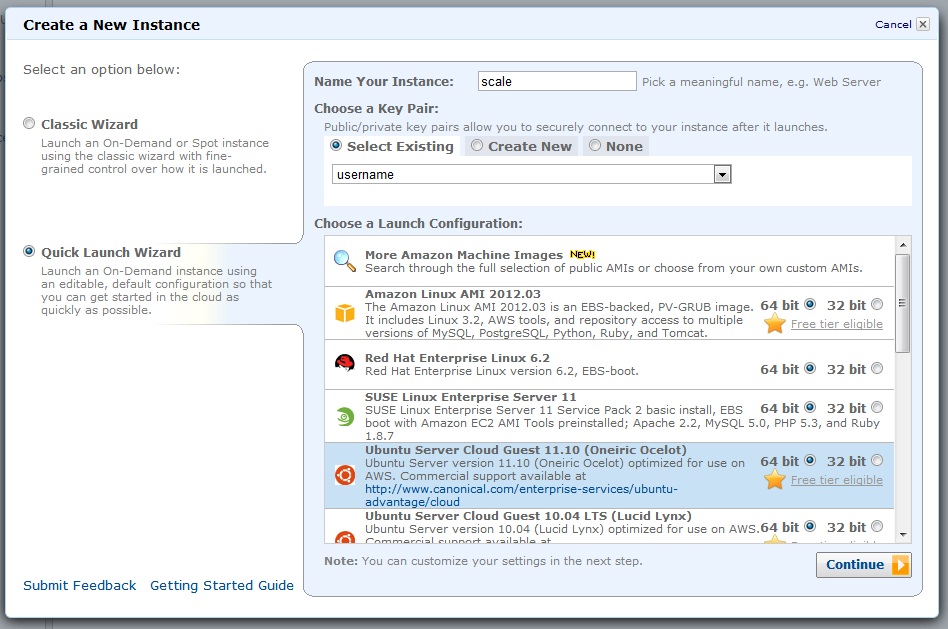
\includegraphics[width=6in]{screen1}

\begin{enumerate*}
\item Name Your Instance: Be creative. Or don't. But name it something
\item Choose a Key Pair: Use an existing pair if you've created one. Otherwise use Create New with Name: your username. Let the key download and remember where it is.
\item Choose a Launch Configuration: Use a modern version of 64-bit Ubuntu Server, preferably one that matches your local configuration.
\item Click ``Continue.''
\end{enumerate*}

\subsubsection*{Screen 2}

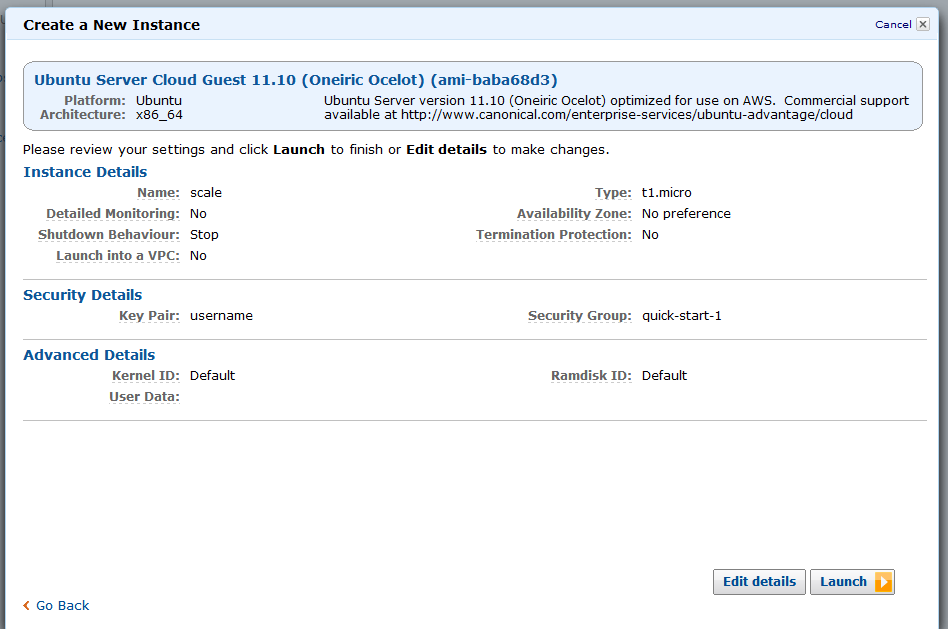
\includegraphics[width=6in]{screen2}

Simply click ``Edit details''

\subsubsection*{Screen 3}

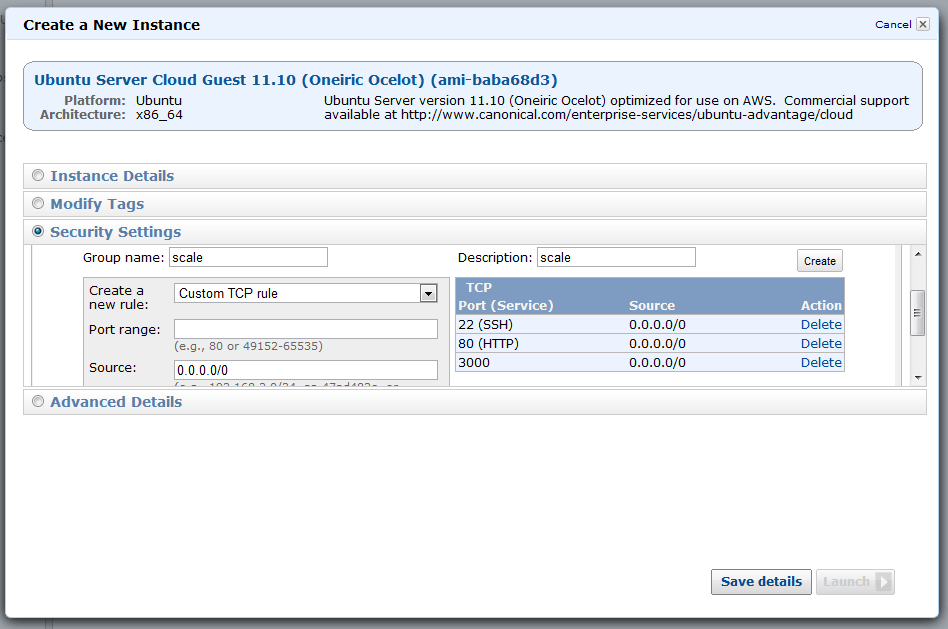
\includegraphics[width=6in]{screen3}

\begin{enumerate*}
\item Instance Details
\begin{enumerate*}
\item Type: t1.micro. Unless you want to actually owe Amazon money
\end{enumerate*}
\item Security Settings - Click ``Create new Security Group''
\begin{enumerate*}
\item Group name/Description: Your call.
\item New rules
\begin{enumerate*}
\item Create a new rule: SSH, HTTP, Custom TCP Rule
\item Port range: n/a, n/a, 3000
\item Source: 0.0.0.0/0
\end{enumerate*}
\item Click ``Create''
\end{enumerate*}
\item Click ``Save details''
\end{enumerate*}

\subsubsection*{Screen 4}

Click ``Launch''

\task{5}{Pairing the Instance}

In this section, we discuss pairing your new EC2 instance with an Elastic IP. Again starting from \href{https://console.aws.amazon.com}{https://console.aws.amazon.com}, do the following:

\begin{enumerate*}
\item Click the ``Amazon EC2'' tab
\item Click ``Elastic IPs'' on the left sidebar
\item Click ``Allocate New Address'' on the top toolbar
\item Click ``Yes, Allocate''
\item Check the box of your new Elastic IP and click ``Associate Address''
\begin{enumerate*}
\item Instance: Select your new EC2 instance.
\item Click ``Yes, Associate''
\end{enumerate*}
\end{enumerate*}

\task{5}{Connecting to the Instance}

Fire up a shell with SSH, and run:

\begin{verbatim}
$ ssh -i <key pair name>.pem ubuntu@<your elastic IP>
\end{verbatim}

\subsection*{Extra Credit}

You may earn extra credit for this lab by adapting the HelloWorld application from earlier labs to work on your AWS account.

\subsection*{Turn-in instructions}
Create a personal Git repository on GitHub named ``Lab\labnumber-username'', where \verb!username! is your Kerberos username, and commit the following files to it:
\begin{itemize}
\item Edited project files from \productname
\item A PDF file with the answers to each question \textit{clearly marked}. When you have completed this lab, you will have answered \total{questions} questions.
\item A \verb!who.txt! file with your name. If you worked with someone else, include their name in the \verb!who.txt! file.
\end{itemize}

Once committed, push all files to GitHub. You may work with a partner, as long as each of you pushes your own copy of all of the listed files. Note that files submitted via ANGEL, email, or other methods will receive zero credit. In addition, files that cannot be accessed without additional work (e.g. zip files, LaTeX documents that require compiling) will lose you points. After you push your files to GitHub, please complete the feedback survey on Angel Under Labs - Labs Anonymous Feedback!


\subsection*{Revision History}
\begin{itemize*}
\item Fri Apr 20 10:29:39 EDT 2012: Lab written by Alex Mullans, Samad Jawaid, and Tim Ekl
\end{itemize*}

\end{document}
